\subsubsection*{A. Azats rounding}

\problemauthor{ Баев А.Ж.}

Достаточно, заметить, что в двоичной системе счисления рациональными будут только числа вида $\frac{1}{2^k}$. Ответ: $k$, если $n = 2^k$, в противном случае ответ равен $(-1)$.

Асимптотика: $O(\log{n})$.

\subsubsection*{B. Billiards}

\problemauthor{ Баев А.Ж.}

Отразим исходный прямоугольник $w \times h$ симметрично относительно каждой из сторон. Полученные прямоугольники  снова отразим зеркально относительной каждой из сторон. Таким образом замостим всю плоскость. Все точки, в которые попадают образы левого нижнего угла исходного прямоугольника, образуют сетку с шагом $(2w, 2h)$. Первое попадание в одну из данных точек прямой $(x, y) \cdot t$ при $t > 0$ и соответствует возврату шара в исходный угол:
$$
\begin{cases}
2 w n = x t\\
2 h m = y t
\end{cases}
$$

\begin{center}
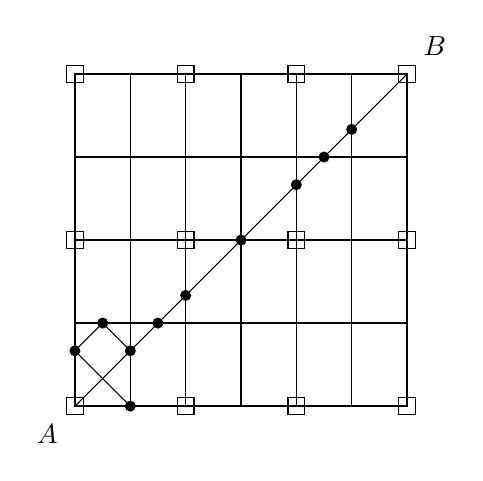
\begin{tikzpicture}[x=10, y=10]
\foreach \x in {0,2,4,6,8,10}
    \foreach \y in {0,3,6,9}  
		\draw[line width=0.5] (\x, \y) rectangle (\x + 2, \y + 3);

\foreach \x in {0,4,8,12}
    \foreach \y in {0, 6,12}  
		\draw (\x - 0.3, \y - 0.3) rectangle (\x + 0.3, \y + 0.3);
		
\draw (0,0) -- (12, 12);
\draw (2,2) -- (1, 3) -- (0, 2) -- (2, 0);
\fill (1, 3) circle (0.2);
\fill (0, 2) circle (0.2);
\fill (2, 0) circle (0.2);

\node at (-1, -1) {$A$};
\node at (13, 13) {$B$};

\fill (2, 2) circle (0.2);
\fill (3, 3) circle (0.2);
\fill (4, 4) circle (0.2);
\fill (6, 6) circle (0.2);
\fill (8, 8) circle (0.2);
\fill (9, 9) circle (0.2);
\fill (10, 10) circle (0.2);
\end{tikzpicture}
\end{center}

Чтобы найти минимальные подходящие $n$ и $m$, поделим данные уравнения:
$$ \frac{m}{n} = \frac{x h}{y w}$$
Пусть $d = (xh, yw)$ --- наибольший общий делитель (можно найти алгоритмом Евклида). Тогда $n = \frac{xh}{d}$, $m = \frac{yw}{d}$. А ответ равен $2n-1$ и $2m - 1$. 

Асимптотика: $O(\log(\max(xh, yw)))$.


\subsubsection*{C. Circles}

\problemauthor{ Баев А.Ж.}

\begin{center}
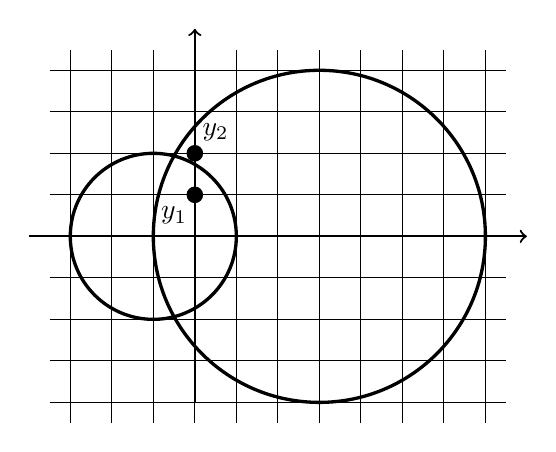
\begin{tikzpicture}[x=15, y=15]
\draw[thick, ->] (-4, 0) -- (8, 0);
\draw[thick, ->] (0, -4) -- (0, 5);
\draw[very thick] (3, 0) circle (4);
\draw[very thick] (-1, 0) circle (2);
\draw[step=1] (-3.5, -4.5) grid (7.5, 4.5);
\fill (0, 1) circle (0.2);
\fill (0, 2) circle (0.2);
\node at (-0.5, 0.5) {$y_1$};
\node at (0.5, 2.5) {$y_2$};
\end{tikzpicture}
\end{center}

Для каждого $x$ можно легко определить максимальное значение $y_1(x)$ такое, что точка $(x, y_1(x))$ попадает во внутренность (или на границу) первого круга (в случае, если $|x - x_1| > r_1$, то таких точек нет вообще и будем считать $y_1(x) = -1$). Это можно сделать не прибегая к вещественной арифметике, с помощью бинарного поиска $y_1(x)$ по ответу от 0 до $r_1 + 1$ с условием, что  $y_1(x)^2 + (x - x_1)^2 \leqslant r^2$. Аналогично находим $y_2(x)$ и находим $y(x) = \min(y_1(x), y_2(x))$. В случае, если $y(x) < 0$, то подходящих точек с абсциссой $x$ нет. Иначе их в точности $2 y(x) + 1$. Таким образом, перебирая все $x$ от $\max(x_1 - r_1, x_2 - r_2)$ до $\min(x_1 + r_1, x_2 + r_2)$ мы найдем ответ.

Асимптотика: $O(r \log r)$.

Замечание: перебор за $O(r^2)$ превышает ограничения по времени.

\subsubsection*{D. Diners}

\problemauthor{ Баев А.Ж.}

Запустим обход в глубину из вершины 1, расставляя у каждой вершины расстояние от корня. Дополнительно найдем $d$ --- максимальную глубину. Далее запустим еще один обход в глубину, при котором для каждой вершины $v$ проверяем, можно ли от нее дойти вглубь до максимальной глубины $d$ или нет. Если дойти можно, а сама вершина находится на глубине $[d/2]$, то эта вершина попадает в ответ.

Асимптотика: $O(n)$.

\subsubsection*{E. Examination aura}

\problemauthor{ Абдикалыков А.К.}

Отсортируем все числа по возрастанию: $b_1 \leqslant b_2 \leqslant ... \leqslant b_n$.

Решение 1. Для каждой пары последовательных вершин $b_{i}$ и $b_{i+1}$ проверяем, хватает ли времени $k_i$, чтобы увеличить все элементы с $b_1$ по $b_i$ до уровня $b_{i+1}$. То есть суммарно увеличить на $(b_{i+1} - b_i) i \leqslant k_{i}$, где $k_{i}$  --- количество часов, оставшихся перед просмотром $i$-го элемента. Если $i = n$ или остается время, чтобы дополнить все элементы до уровня $a_{i+1}$, то уменьшаем оставшееся время: $k_{i+1} = k_i - (a_{i+1} - a_i) i$. В противном случае выводим ответ $a_i + [k_i / i]$.

Асимптотика: $O(n\ log n)$.

Решение 2. Фиксируем $a$ --- минимальный уровень, до которого увеличиваем все элементы $b_i < a$. Проверяем, хватит ли времени $k$ для соответствующих элементов: $\sum_{i = 0}^{n} \max(a - b_i, 0) \leqslant k$. Для нахождения максимального подходящего уровня используем бинарный поиск по ответу от 0 до $\max{b_i}$, 

Асимптотика: $O(n (\log n + \log a))$.

\subsubsection*{F. Fibonaccissimo}

\problemauthor{ Баев А.Ж.}

Числа Фибоначчи с большим индексом можно найти в результате возведения в степень матрицы:
$$
\begin{pmatrix}
F_{n+1} & F_{n} \\
F_{n} & F_{n-1}
\end{pmatrix}
=
\begin{pmatrix}
1 & 1 \\
1 & 0
\end{pmatrix}^n
$$

Причем сделать это можно бинарным возведением в степень:
$$A =
\begin{cases}
\left(A^{n/2}\right)^2, \text{ если n --- четное положительное,} \\
A \cdot \left(A^{n/2}\right)^2, \text{ если n ---нечетное ,} \\
E, n = 0
\end{cases}
$$

Проблема заключается в том, что само $F_n$ не помещается стандартный тип. Докажем, что при возведении в степень матрицы Фибоначчи по модулю $10^9+9$ можно использовать аналог малой теоремы Ферма, что позволит значительно упростить нахождение ответа.

Несложно убедиться, что существует такой элемент $x$, что $x^2 \equiv 5 \bmod (10^9+9)$. Значит, существуют элементы $\sqrt{5}$, $\lambda_1 = \frac{1 +\sqrt{5}}{2}$ и $\lambda_2 = \frac{1 -\sqrt{5}}{2}$ по модулю $10^9+9$. По аналогии с полем вещественных чисел матрицу можно привести к диагональному виду следующим образом:
$$
\begin{pmatrix}
1 & 1 \\
1 & 0
\end{pmatrix}
=
\frac{1}{\sqrt{5}}
\begin{pmatrix}
1 & 1 \\
-\lambda_2 & -\lambda_1
\end{pmatrix}
\begin{pmatrix}
\lambda_1 & 0 \\
0 & \lambda_2
\end{pmatrix}
\begin{pmatrix}
\lambda_1 & 1 \\
-\lambda_2 & -1
\end{pmatrix}
=
G \Lambda G^{-1}
$$
Тогда ясно, что возведение в степень сводится к возведению в степень диагональной матрицы:
$$
\begin{pmatrix}
1 & 1 \\
1 & 0
\end{pmatrix}^k
=
\frac{1}{\sqrt{5}}
\begin{pmatrix}
1 & 1 \\
-\lambda_2 & -\lambda_1
\end{pmatrix}
\begin{pmatrix}
\lambda_1^k & 0 \\
0 & \lambda_2^k
\end{pmatrix}
\begin{pmatrix}
\lambda_1 & 1 \\
-\lambda_2 & -1
\end{pmatrix}
=
G \Lambda^k G^{-1}
$$

А для диагональных элементов матрицы применима малая теорема Ферма $\lambda^{p-1} \equiv 1 \bmod p$. Значит, малая теорема Ферма применима при возведении в степень данной матрицы по данному модулю.

Теперь можно быстро возводить в степень:
$$A^k \equiv A^{k \bmod (p-1)} \bmod p.$$
Во--первых, с помощью матричного возведения находим $k = F_n \bmod (p-1)$. Во--вторых, находим $F_{F_n} = F_k \bmod p$.

Асимптотика: $\log {n}$.

Замечание: малая теорема Ферма по модулю $p$ для целочисленных матриц выполняется в том случае, если все собственные значения матрицы существуют по модулю $p$.

\subsubsection*{G. Good round numbers}

\problemauthor{ Абдикалыков А.К.}

Ответом на задачу является значение $D(b) - D(a-1)$, где $D(m)$ --- количество подходящих чисел среди чисел от $1$ до $m$. Чтобы найти числа с круглостью $c$ достаточно перебрать числа вида $n(n+c)$ (это можно сделать за $O(\sqrt{m})$). При этом не забыть отбросить те из них, которые имеют другое разложение $n_1(n_1 + c_1)$, где $c_1 < c$.  Несложно убедиться, что все числа вида $n^2$, $n(n+1)$ и $n(n+2)$ имеют круглость 0, 1 и 2 соответственно. У чисел вида $n(n+3)$ имеется единственное исключение: $4 = 1 \cdot (1 + 3) = 2 \cdot 2$, которое имеет круглость 0. У чисел вида $n(n+4)$ имеется тоже единственное исключение: $12 = 2 \cdot 6 = 3 \cdot 4$, которое имеет круглость 1.

Асимптотика: $O(\sqrt {B})$.

Замечание: при более существенных ограничениях на $C$ асимптотика будет равна $O(C \sqrt {B})$.

\subsubsection*{H. Hit a ball}

\problemauthor{ Абдикалыков А.К.}

Во всех других задачах можно было найти явные намеки на круги, сферы и шары. В самой задаче можно было посчитать количество слов между запятыми: 3 1 4 1 5 9 ... Название задачи состояло из слов 3, 1 и 4 буквами. Ответ: соответствующая цифра числа $\pi$.

Асимптотика: $O(1)$.

\subsubsection*{I. Incalculable result}

\problemauthor{ Нуразханов Ч.}

Промоделируем процесс для первых $\max (a_i + 2, 2 k)$ игр (учитывая условия можно было промоделировать 1001 шаг). Игра будет некорректной в двух случаях: либо выигрыш серии наступил до последней неожиданной игры $a_n$; либо после последней неожиданной игры разница $a_n$, разница в счете начинает повторятся (то 0, то 1).

Асимптотика: $O(\max{a_i})$.
